\documentclass[12pt,a4paper]{article}
\usepackage[UTF8]{ctex}
\usepackage{amsmath,amssymb}
\usepackage{xcolor}
\usepackage{hyperref}
\usepackage{geometry}
\usepackage{graphicx}
\geometry{margin=2.5cm}

\title{Quantum Teleportation}
\author{QuoNic}
\date{}

\begin{document}
\maketitle

\begin{center}
\textbf{Communication} | Difficulty: Intermediate | Time: 10 min
\end{center}

\tableofcontents
\newpage

\section{Why do we need it?}

Quantum teleportation can transfer quantum states without directly transmitting qubits. This is the core protocol of quantum communication.

\subsection{Classical Limitations}
\begin{itemize}
  \item Classical communication cannot transmit quantum states (no-cloning theorem)
  \item Direct qubit transmission is vulnerable to noise and decoherence
\end{itemize}

\subsection{Quantum Advantages}
\begin{itemize}
  \item Uses entanglement and classical communication to transfer quantum states
  \item Does not violate no-cloning theorem (original state is destroyed)
  \item Foundation for quantum networks
\end{itemize}

\subsection{Real-world Applications}
\begin{itemize}
  \item Quantum Networks (quantum internet)
  \item Distributed Quantum Computing
  \item Quantum Key Distribution
\end{itemize}

\section{Quick Start}

\begin{verbatim}
import math
from quonic import qgate, qshow
from quonic.gates import CX, CZ, H, Ry

# Prepare state to teleport
qgate(Ry(math.pi / 3), 0)

# Create Bell pair
qgate(H, 1)
qgate(CX, 1, 2)

# Alice's operations
qgate(CX, 0, 1)
qgate(H, 0)

# Bob's corrections
qgate(CX, 1, 2)
qgate(CX, 0, 2)
qgate(CZ, 0, 2)

qshow()
\end{verbatim}

\textbf{Expected Output}:
\begin{verbatim}
backend: native | shots: 1024
Result:
  |000>    256  ( 25.0%)  ##########
  |010>    256  ( 25.0%)  ##########
  |100>    256  ( 25.0%)  ##########
  |110>    256  ( 25.0%)  ##########
\end{verbatim}

\section{Theory Deep Dive}

\subsection{Circuit Diagram}

\begin{center}
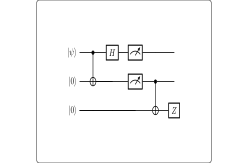
\includegraphics[width=0.7\textwidth]{../../images/teleportation_circuit.svg}
\end{center}

\subsection{Mathematical Derivation}

\textbf{Step 1: Prepare State}

Alice has $q_0$ in state $|\psi\rangle = \cos(\pi/6)|0\rangle + \sin(\pi/6)|1\rangle$

\textbf{Step 2: Create Bell Pair}

Alice and Bob share Bell pair:
\begin{equation}
|\Phi^+\rangle_{12} = \frac{|00\rangle + |11\rangle}{\sqrt{2}}
\end{equation}

\textbf{Step 3: Alice's Operations}

Alice applies CNOT and $H$ gates to $q_0$ and $q_1$.

\textbf{Step 4: Measurement}

Alice measures $q_0$ and $q_1$, getting 2 classical bits $(a, b)$:
\begin{itemize}
  \item $(0,0)$: $q_2 = |\psi\rangle$ (no correction needed)
  \item $(0,1)$: $q_2 = X|\psi\rangle$ (apply $X$ gate)
  \item $(1,0)$: $q_2 = Z|\psi\rangle$ (apply $Z$ gate)
  \item $(1,1)$: $q_2 = XZ|\psi\rangle$ (apply $X$ and $Z$ gates)
\end{itemize}

\textbf{Step 5: Bob's Correction}

Bob corrects $q_2$ based on Alice's measurement results.

\textbf{Step 6: Result}

$q_2$ is now in state $|\psi\rangle$, completing quantum state transfer.

\subsection{Geometric Interpretation}

Quantum teleportation uses entanglement as a quantum channel to transfer quantum states without directly transmitting qubits.

\section{Code Walkthrough}

\begin{verbatim}
import math
from quonic import qgate, qshow
from quonic.gates import CX, CZ, H, Ry

# Step 1: Prepare state to teleport
qgate(Ry(math.pi / 3), 0)  # q0 = cos(pi/6)|0> + sin(pi/6)|1>

# Step 2: Create Bell pair
qgate(H, 1)      # q1 -> (|0>+|1>)/sqrt(2)
qgate(CX, 1, 2)  # q1,q2 -> (|00>+|11>)/sqrt(2)

# Step 3: Alice's operations
qgate(CX, 0, 1)  # CNOT(q0, q1)
qgate(H, 0)       # H(q0)

# Step 4: Bob's corrections
qgate(CX, 1, 2)  # CNOT(q1, q2)
qgate(CX, 0, 2)  # CNOT(q0, q2)
qgate(CZ, 0, 2)  # CZ(q0, q2)

qshow()
\end{verbatim}

\section{Advanced Usage}

\subsection{Scenario 1: Teleport Different States}

\begin{verbatim}
# Teleport |0>
qgate(Ry(0), 0)
# ... teleportation protocol ...

# Teleport |1>
qgate(Ry(math.pi), 0)
# ... teleportation protocol ...

# Teleport |+>
qgate(H, 0)
# ... teleportation protocol ...
\end{verbatim}

\subsection{Scenario 2: Noisy Teleportation}

\begin{verbatim}
# No noise
qshow(noise=0)

# 5% noise
qshow(noise=0.05)

# 20% noise
qshow(noise=0.20)
\end{verbatim}

\section{Use Cases}

\subsection{Quantum Networks}

Quantum teleportation is the foundation of quantum networks, enabling quantum state transfer between nodes.

\subsection{Distributed Quantum Computing}

In distributed quantum computing, teleportation transfers quantum states between different quantum processors.

\subsection{Quantum Key Distribution}

Teleportation can be used for quantum key distribution, enabling secure key transfer.

\section{FAQ}

\subsection{Can teleportation enable faster-than-light communication?}

No. Teleportation requires classical communication to transmit measurement results, which is limited by the speed of light.

\subsection{Does teleportation violate the no-cloning theorem?}

No. Teleportation destroys the original state, so it does not violate the no-cloning theorem.

\subsection{How many qubits does teleportation need?}

3 qubits: 1 state to teleport + 2 Bell pair qubits.

\subsection{What is the fidelity of teleportation?}

Ideally 1. In practice, noise reduces fidelity.

\subsection{What's the relationship between teleportation and quantum repeaters?}

Quantum repeaters use teleportation and entanglement swapping for long-distance quantum communication.

\section{Learning Path}

\subsection{Prerequisites}
\begin{itemize}
  \item Bell state (2-qubit entanglement)
  \item CNOT gate and Hadamard gate
  \item Quantum measurement
\end{itemize}

\subsection{Next Steps}
\begin{itemize}
  \item Superdense Coding (transfer classical info using Bell states)
  \item Quantum Repeaters (long-distance quantum communication)
  \item Quantum Networks (quantum internet)
\end{itemize}

\section{Complete Examples}

\subsection{Example 1: Basic Teleportation}

\begin{verbatim}
import math
from quonic import qgate, qshow
from quonic.gates import CX, CZ, H, Ry

qgate(Ry(math.pi / 3), 0)
qgate(H, 1)
qgate(CX, 1, 2)
qgate(CX, 0, 1)
qgate(H, 0)
qgate(CX, 1, 2)
qgate(CX, 0, 2)
qgate(CZ, 0, 2)
qshow()
\end{verbatim}

\section{Download}

\begin{itemize}
  \item [teleportation.py](https://github.com/ChrisLee0721/QuoNic/blob/main/examples/teleportation/teleportation.py)
\end{itemize}

\end{document}
